\documentclass[twoside,letterpaper,11pt]{article}

\usepackage{graphicx}

\usepackage{amsthm}
\newtheorem{mydef}{Definition}

\begin{document}
\setlength{\pdfpageheight}{\paperheight}
\setlength{\pdfpagewidth}{\paperwidth}

\title{Causal vs. Temporal Learning}
\author{Bo Morgan\\
MIT Media Lab}
\renewcommand{\today}{September 26, 2011}
\maketitle


%\section{}

%Jim Bleights PRODIGY (planner called Weaver had conditional effects).

\section{The Planning Task}

[To do: Make this definition of the planning task allow for state dependent effects of operators.]

\begin{mydef}
A planning task is a 4-tuple $\Pi~=~{\langle}V,O,I,G{\rangle}$, where

\begin{itemize}
\item $V$ is a finite set of \emph{propositional state variables} (also called \emph{propositions} or \emph{facts}),
\item $O$ is a finite set of \emph{operators}, each with associated \emph{preconditions} $pre(o)~\in~V$, \emph{add effects} $add(o)~\in~V$ and \emph{delete effects} $del(o)~\in~V$,
\item $I~\in~V$ is the \emph{initial state}, and
\item $G~\in~V$ is the set of \emph{goals}.
\end{itemize}

\end{mydef}

A \emph{state} is a subset of facts, $s~\in~V$, representing the propositions which are currently true.
\emph{Applying} an operator $o$ in $s$ results in state $(s~\setminus~del(o))~\cup~add(o)$, which we denote as $s[o]$.
The notation is only defined if $o$ is \emph{applicable} in $s$, i.e., if $pre(o)~\in~s$.
Applying a sequence $o_1,{\ldots},o_{n+1}$ of operators to a state is defined inductively as $s[\epsilon]~:=~s$ and $s[o_1,{\ldots},o_{n+1}]~:=~(s[o_1,{\ldots},o_n])[o_{n+1}]$.
A plan for a state $s$ (\emph{s-plan} or \emph{plan} when $s$ is clear from context) is an operator sequence $\pi$ such that $s[\pi]$ is defined and satisfies all goals (i.e., $G~\in~s[\pi]$).


\section{Learning the Effects of Planning Operators}

We would like our system to be able to adapt to novel environments.
Toward this end, we allow for $s[o]$ and $pre(o)$ to be learned during the run-time of the system.

\section{Concept Learning and Hypothesis Spaces}

If some instance $x$ satisfies all the constains of hypothesis $h$, then $h$ classifies $x$ as a positive example ($h(x)~=~1$).
The set of items over which the concept is defined is called the set of \emph{instances}, which we denote by $X$.
The concept or function to be learned is called the \emph{target concept}, which we denote by $c$.
In general, $c$ can be any boolean-valued function defined over the instances $X$; that is, $c~:~X~\rightarrow~\{0,1\}$.
When learning the target concept, the learner is presented a set of \emph{training examples}, each consisting of an instance $x$ from $X$, along with its target concept value $c(x)$.
Instances for which $c(x)~=~1$ are called \emph{positive examples}, or members of the target concept.
Instances for which $c(x)~=~0$ are called \emph{negative examples}, or nonmembers of the target concept.
We use the symbol $D$ to denote the set of available training examples.


\begin{mydef}
Let $h_j$ and $h_k$ be boolean-valued functions defined over $X$.
Then $h_j$ is \emph{more general than or equal to} $h_k$ (written $h_j~{\geq}_g~h_k$) if and only if

\begin{equation}
({\forall}x \in X)[(h_k(x) = 1) \rightarrow (h_j(x) = 1)]
\end{equation}

\end{mydef}


\section{Learning to make planning decisions}

Learning to make planning decisions is an example of a delayed
learning task, where the category to be learned is not available at
the same time that the features are available.  For example, plans
that are successful in accomplishing types of goals will also tend to
be developed through similar types of planning.  Heuristics can be
learned to predict actual success or failure from features of the
planning space.  Then, we use these heuristics to guide the planning
search, less completely toward a static heuristic of plan distance and
more toward a learned heuristic based on types of execution successes
and failures.

\subsection{The problem with pyramids}

In our block building toy problem we have cubic blocks and pyramidal
blocks.  The gripper is able to pick up cubic blocks, while pyramidal
blocks are impossible for the gripper to pick up.  The gripper has two
sources of knowledge for accomplishing the given goal.  Knowledge is a
causal relationship between states, or in other words, an action
trans-frame.  These two knowledge sources have features that can be
used for training our heuristics.  

The block building domain is shown in
Figure~\ref{fig:block_building_domain}, where four panels (a, b, c, d)
illustrate a scenario of learning to make planning decisions.

\begin{figure}[here]
\centering
a.~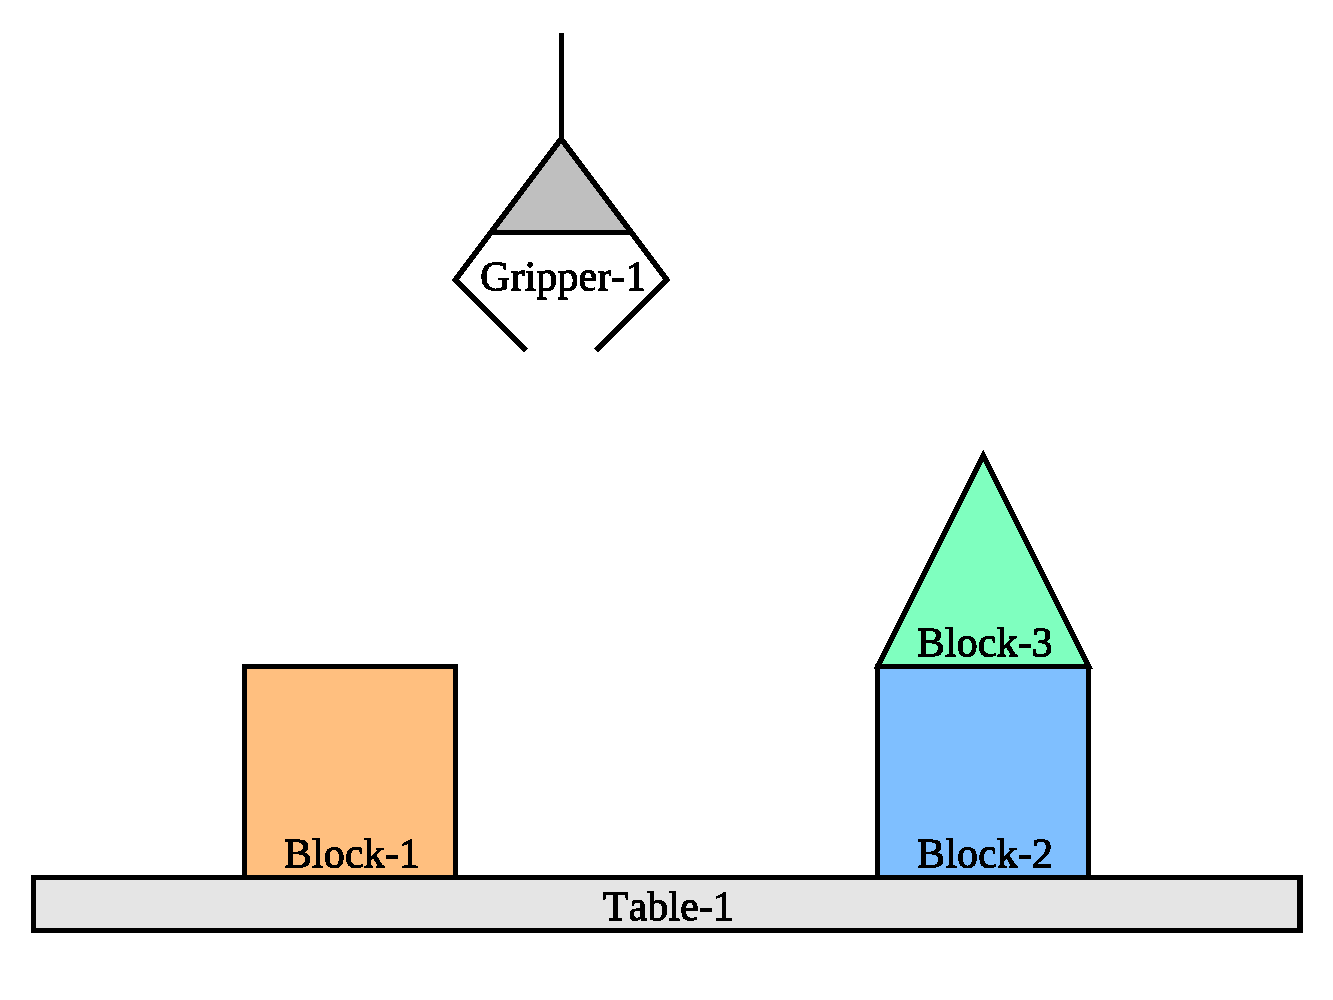
\includegraphics[width=0.4\textwidth]{block_building-1}~~b.~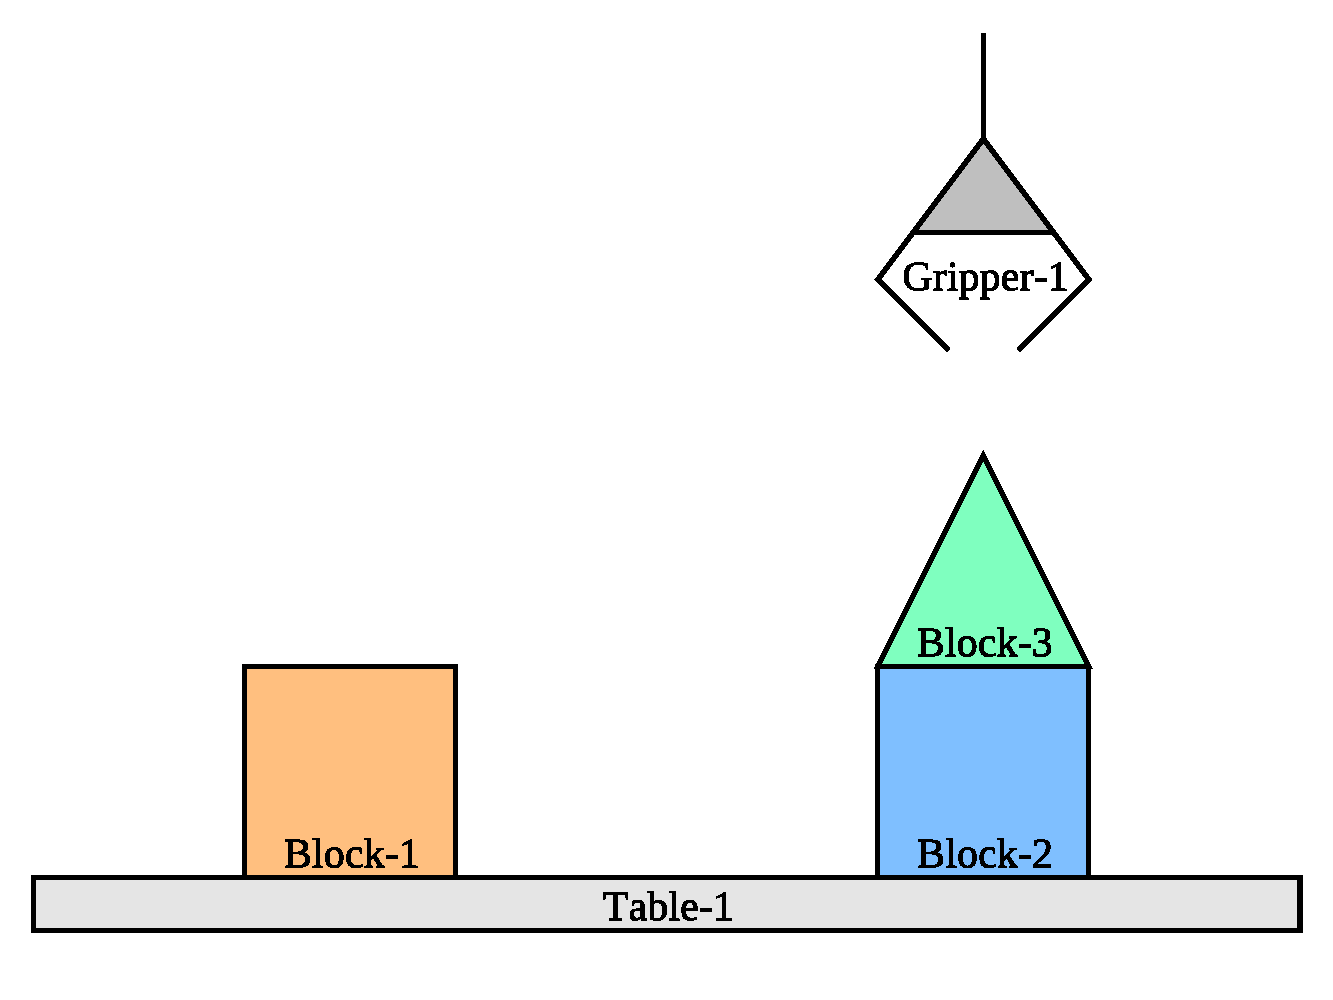
\includegraphics[width=0.4\textwidth]{block_building-2}

c.~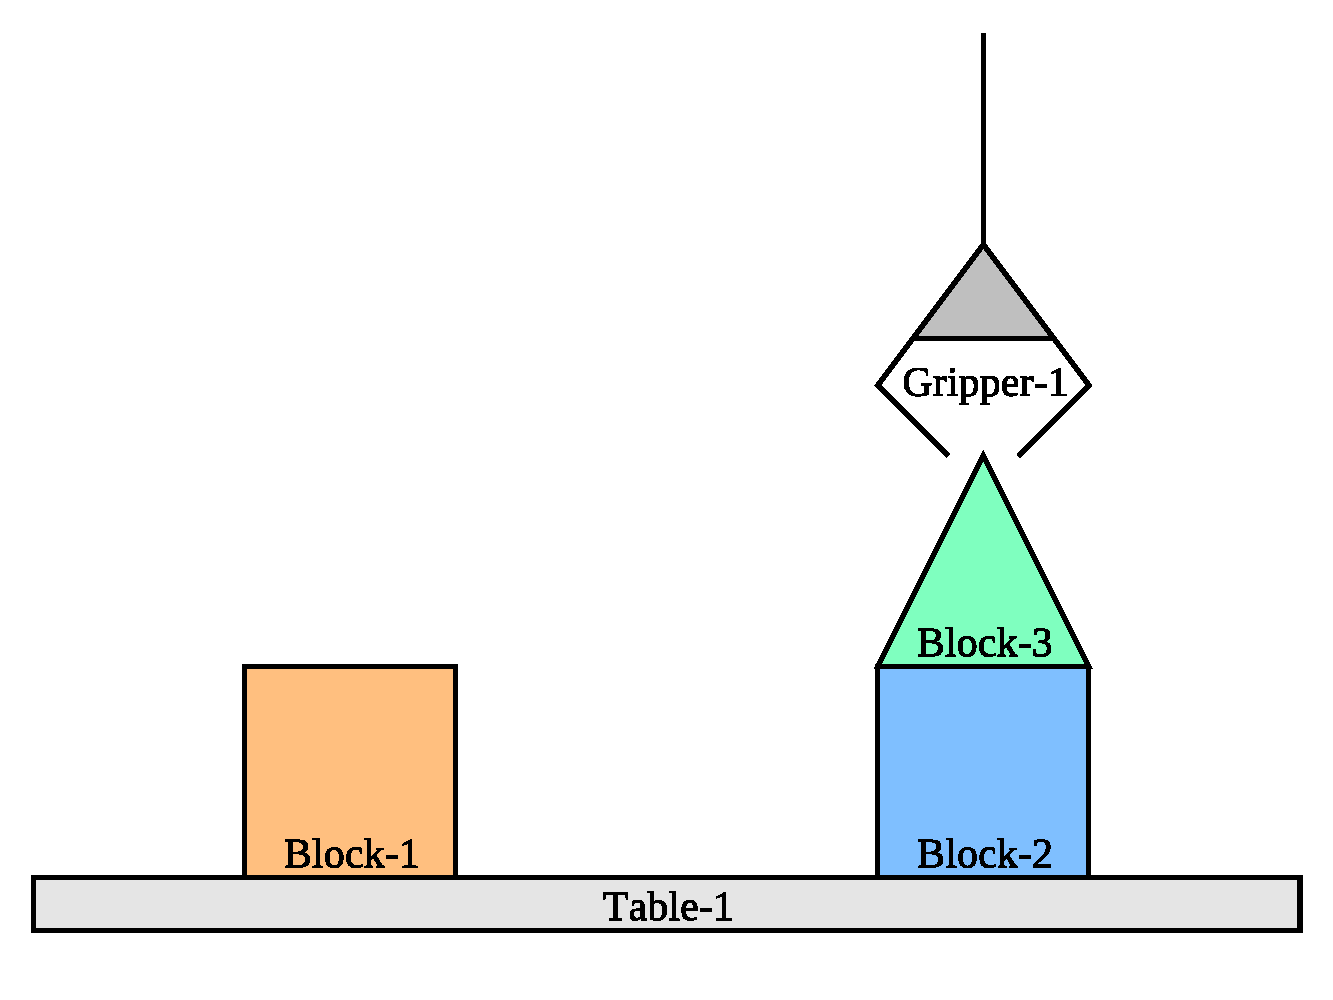
\includegraphics[width=0.4\textwidth]{block_building-3}~~d.~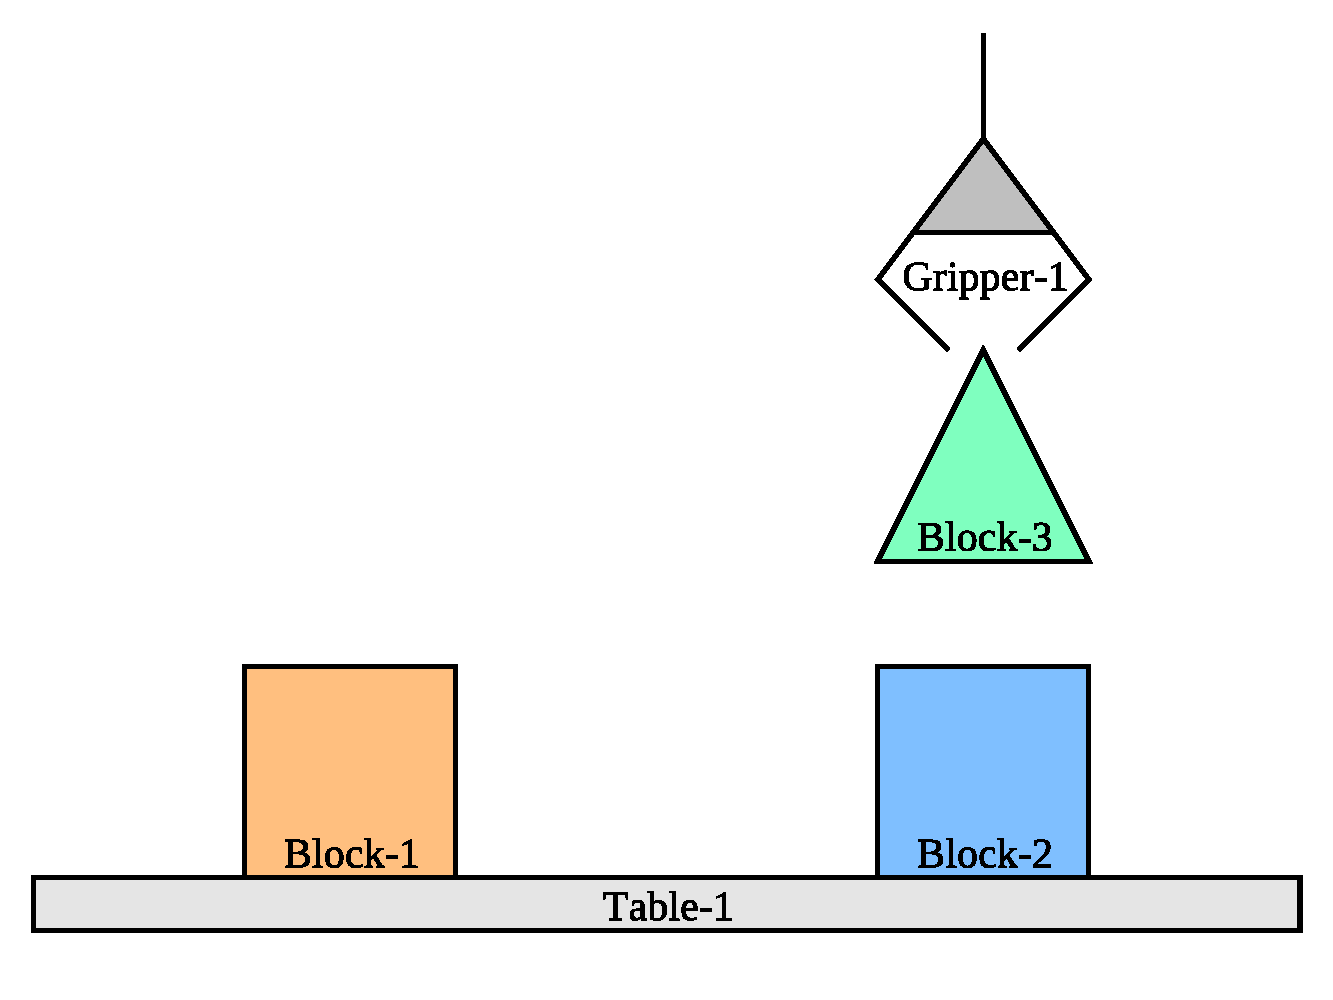
\includegraphics[width=0.4\textwidth]{block_building-4}
\caption{Block building domain.  (\emph{a}) the initial starting
  physical state of the gripper in the block building domain.
  (\emph{b}) how a planning process could represent the result if the
  gripper were to \emph{move right}.  (\emph{c}) how a planning
  process could represent the result if the gripper were to try to
  \emph{grab} the block below.  (\emph{d}) how a planning process
  could misrepresent the later result if the gripper were to try to
  \emph{grab} the block below.  }
\label{fig:block_building_domain}
\end{figure}





\subsection{Correct Knowledge}

\subsection{Incorrect Knowledge}



\section{A Concrete Plan}


%Feedback from Committee:
%
%  Needed by Wednesday:
%
%    -- A plan that says what I'll do.
%    -- What tests I will run and how I intend to interpret the results.
%    -- Preferably: A revised outline of the thesis.
%
%    For the Implementation:
%
%      -- Show dense reflective traceback.
%
%        -- For example, I need to show the traceback working when the
%           system encounters a realistic bug.
%
%        -- I should also show how this traceback data would be used to
%           revise execution.
%
%    For the Thesis:
%
%      -- Make the thesis clear in the document from the outset, and
%         stick to these ideas throughout.
%
%MY ADVICE IS TO DEVELOP A SIMPLE AND CLEAR NARRATIVE RUNNING FROM YOUR CONTRIBUTIONS TO YOUR IMPLEMENTATION THROUGH YOUR THEORY. YOU START VERY SIMPLE AND DEVELOP IT BY ADDING TECHNICAL DETAIL AS YOU PROCEED. TO DO THIS, IT IS IMPORTANT TO DETERMINE WHAT YOU WILL *NOT* SAY AS MUCH AS WHAT YOU WILL SAY. 
%
%        -- Use the defense material for focus.
%
%        -- Make clear what has been implemented.
%

\subsection{Credit Assignment Metric}

  First, I will develop a metric by which I can measure the
  performance of my credit assignment algorithm versus other
  algorithms.  At one extreme, we have the brute force approach to
  learning, in which all possible concepts are re-learned at every
  opportunity (e.g. at every step in a Markov stepped system, or at
  every knowledge event in my real-time event driven system).  At the
  other extreme, we re-learn only those concepts whose fundamental
  training knowledge has changed (instances, hypothesis space, or
  features).  My approach to tracing the provenance of deliberative
  knowledge through the reactive plan execution agencies will be
  somewhere between these two extremes of efficiency.


  -- Evaluation Metrics

     -- credit assignment: the process of choosing a subset from the
                           total possible set of concepts that should
                           be focused on as being responsible for the
                           occurrence of a given event.

EXACTLY WHAT IS THE METRIC HERE? HOW WILL IT BE MEASURED? YOU HINT AT SPEED BELOW, AND IF THIS IS TRUE, WILL IT BE MEASURED IN DECISION-CYCLE TIME? DEFINE AND OPERATIONALIZE YOUR METRIC.

       The credit assignment process can be more or less efficient in
       focusing the learning resources toward concepts that can be
       re-learned.

\subsection{Temporal Credit Assignment}

       I can measure the performance of my causal credit assignment
       algorithm versus a typical temporal credit assignment
       algorithm, such as an adaptation of the Temporal Difference
       (TD) learning algorithm commonly used in the field of
       reinforcement learning.

HAVE YOU ALREADY IMPLEMENTED THIS ALGORITHM? WILL YOU USE AN EXISTING IMPLEMENTATION?

\subsection{Causal Credit Assignment}

        The goal of these tests are to show that learning by
        provenance speeds the standard temporal credit assignment
        method, which assigns credit to the sequence of immediately
        previous states and actions.

ABOVE YOU MENTION YOUR CREDIT ASSIGNMENT *VERSUS* A STANDARD ALGORITHM. HERE YOU STATE THAT YOUR VERSION WILL ACCELERATE THE STANDARD ALGORITHM. DO YOU MEAN THAT YOURS IS FASTER THAT THE STANDARD IN THE LIMIT? OR DO YOU INTEND TO COMBINE THEM TO SPEED UP THE TEMPORAL ALGORITHM? 

     -- I will focus on re-learning category concepts given new
        training instances that would change those concepts.

  -- Now, given the above metric for what I will actually be measuring
     as a performance metric, here are two specific deliberative
     learning tasks where my causal learning will be superior to a
     temporal credit assignment method.  This is primarily due to the
     delayed time between deliberation about knowledge and the
     execution of that knowledge, resulting in a precondition check
     form of failure.  Specifically, the precondition check could
     simply be what would be Removed by a trans-frame, but doesn't
     necessarily exist in the physical knowledge at the time of
     execution.  The following are two examples of scenarios:

\subsection{The Social Knowledge Trust Task}

        Some plans can be learned through a social communication
        language.  Physical plans are added to the deliberative
        knowledge with the added relationship with the appropriate
        social provenance markers, e.g. Gripper-1 may represent that a
        given plan is told to it by The-User (or another social
        source).

        The Decision to use a plan that accomplishes a given goal from
        one knowledge source or another can be learned, but the
        learning of this type of action is difficult because of the
        often indirect temporal connection between this deliberative
        Decision involved in choosing or creating a plan and the
        actual execution failure, resulting from executing a plan that
        has derived from that deliberative decision.

THIS LONG RUN-ON SENTENCE IS TYPICAL OF YOUR WRITING AND PLACES THE BURDEN OF UNDERSTANDING UPON THE READER. WHAT IS LEARNED? A DECISION OR AN ACTION? FURTHERMORE, YOU PREVIOUSLY DISCUSSED LEARNING CONCEPTS. IMPLEMENT A SINGLE LEARNING ALGORITHM AND USE IT TO ILLUSTRATE YOUR THEORY. AGAIN, DECIDE WHAT YOU WILL NOT SAY.

\end{document}

